\documentclass{article}[18pt]
\usepackage{../../../../../format}
\lhead{CT - Graphs}


\begin{document}
\begin{center}
\underline{\huge Graph Colouring}
\end{center}
\section{Problems in natural science}
\begin{itemize}
\item Aim: Solve a "real world" problem
\item How: most times it is difficult to try "real world" solutions until we find the best one
\item Therefore
\begin{itemize}
\item We rephrase the problem as an "abstract" problem
\item This is called abstract modelling
\item We can easily
\begin{itemize}
\item Try many alternative solutions to the abstract problem
\item and then "translate" these solutions in terms of the original "real world problem
\end{itemize}
\end{itemize}
\item Usually the "abstract model" involves graphs/networks
\end{itemize}
\section{Radio Frequency assignment}
\begin{itemize}
\item A network of radio transmitters
\item Each of them must have an operating frequency
\item if two nearby transmitters have the same frequency they \textbf{interfere} with each other
\item We \textbf{pay} for every frequency we are using
\item areal world problem: assign the frequencies such that:
\begin{itemize}
\item no transmitters interfere
\item we pay as little as possible
\end{itemize}
\end{itemize}
\begin{itemize}
\item To solve the problem, we do not have to deal with the transmitters themselves
\item We consider a graph problem
\begin{itemize}
\item transmitter $\leftrightarrow$ vertex
\item one edge between two nearby transmitters
\item frequency of transmitter $\leftrightarrow$ colour of its vertex
\end{itemize}
\item Our goal becomes graph colouring
\begin{itemize}
\item assign the smallest number of colours to vertices where two connected vertices have different colour
\end{itemize}
\end{itemize}
\section{Scheduling of talks}
\begin{itemize}
\item A conference agency organises a set of business meetings
\item each meeting has pre-defined start/finish times
\item A hotel room can be used for many meetings, if they do not overlap
\item The agency \textbf{pays} for every hotel room they book
\item Real world problem: book hotel rooms such that:
\begin{itemize}
\item All meetings take place
\item The agency pays as little as possible
\end{itemize}
\end{itemize}
\begin{itemize}
\item Let the meetings have the following start/finish times:
\begin{center}
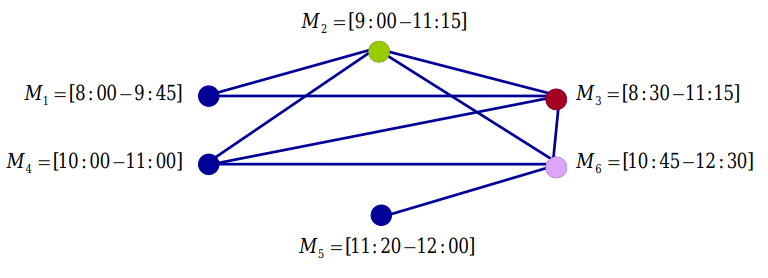
\includegraphics[scale=0.7]{graph}
\end{center}
\item Again, we consider a \textbf{graph colouring problem}:
\begin{itemize}
\item meeting $\leftrightarrow$ vertex
\item one edge between two overlapping meetings
\item room for a meeting $\leftrightarrow$ colour of its vertex
\end{itemize}
\end{itemize}
\section{Timetable of exams}
\begin{itemize}
\item each exam takes one day
\item two exams can be held concurrently if no student is registered in both of them
\item Real world problem: create a timetable such that:
\begin{itemize}
\item each student participates in all his/her exams
\item The exams \textbf{finish as soon as possible}
\end{itemize}
\item Again we consider a graph colouring problem:
\begin{itemize}
\item exam $\leftrightarrow$ vertex
\item one edge between two exams with common students
\item Date of an exam $\leftrightarrow$ colour of its vertex
\end{itemize}
\end{itemize}
\section{Graph colouring}
All these problems (and many others) can be "rephrased" in terms of graph colourings, where:
\begin{itemize}
\item The vertices correspond to transmitters, meetings, exams,...
\item The colours correspond to frequencies, rooms, dates,...
\end{itemize}
But always:
\begin{itemize}
\item The edges correspond to some kind of \textbf{conflicts} (nearby transmitters, overlapping meetings, common students,...)
\end{itemize}
\begin{itemize}
\item In general, it is hard (NP-complete) to compute the smallest number of colours needed for a given graph
\item However, in special cases it is easy:
\begin{itemize}
\item What an graph is a path:
\begin{center}
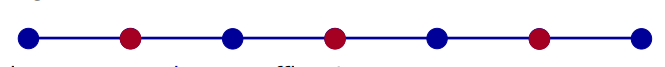
\includegraphics[width=0.7\linewidth]{path}
\end{center}
always two colours suffice
\item When a graph is \textbf{complete} with k vertices
\begin{center}
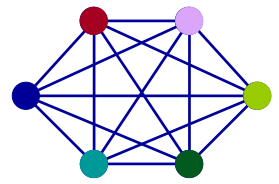
\includegraphics[scale=0.7]{complete}
\end{center}
always k colours needed (every vertex is a different colour)
\end{itemize}
\item Thus, if a graph includes a \textbf{complete subgraph} with \textbf{k vertices}
\begin{itemize}
\item We need at least k colours for this graph
\item When a graph is complete with k vertices, k colours are always needed (each vertex a different colour)
\end{itemize}
\end{itemize}
\section{A simple algorithm}
How to check whether 3 colours are enough?
\begin{itemize}
\item The simplest algorithm: "brute force", i.e. enumerate exhaustively \textbf{all possible 3-colourings} until you:
\begin{itemize}
\item either find a 3-colouring, where any two adjacent vertices have different colours
\item or otherwise conclude that you need more colours
\end{itemize}
\end{itemize}
\begin{center}
\includegraphics[scale=0.7]{"brute force"}
\end{center}
Let's count how many steps we need (for n vertices)
\begin{itemize}
\item 3 choices for the 1st vertex, 3 choices for the 2nd vertex and so on
\item All together $3^n$ steps, which is too many
\end{itemize}
\section{A more "delicate" algorithm}
We can "refine" our search of a good colouring:
\begin{itemize}
\item If two vertices a and b are \textbf{not connected}, then in the optimal colouring:
\begin{enumerate}
	\item either a and b have \textbf{different} colours
	\item if a and b have the \textbf{same} colour
\end{enumerate}
\item In the first case: we can just add an edge between the vertices a and b
\begin{center}
\includegraphics[scale=0.7]{"first case"}
\end{center}
\item In the second case: we can just "merge" the two vertices a and b into one
\begin{center}
\includegraphics[scale=0.7]{"first case1"}
\end{center}
\end{itemize}
This algorithm in action:
\begin{itemize}
\item At every iteration:
\begin{itemize}
\item pick up a pair of non connected vertices a and b
\item try both possibilities a and b have
\begin{itemize}
\item the same colour
\item different colours
\end{itemize}
\item For each case, iterate: find another pair of non connected vertices, iterate ...
\end{itemize}
\item Stop when \textbf{no iteration} is possible i.e. when we end up only with complete graphs
\item The smallest size of these complete graphs is equal to the smallest number of colours we need
\end{itemize}
\begin{center}
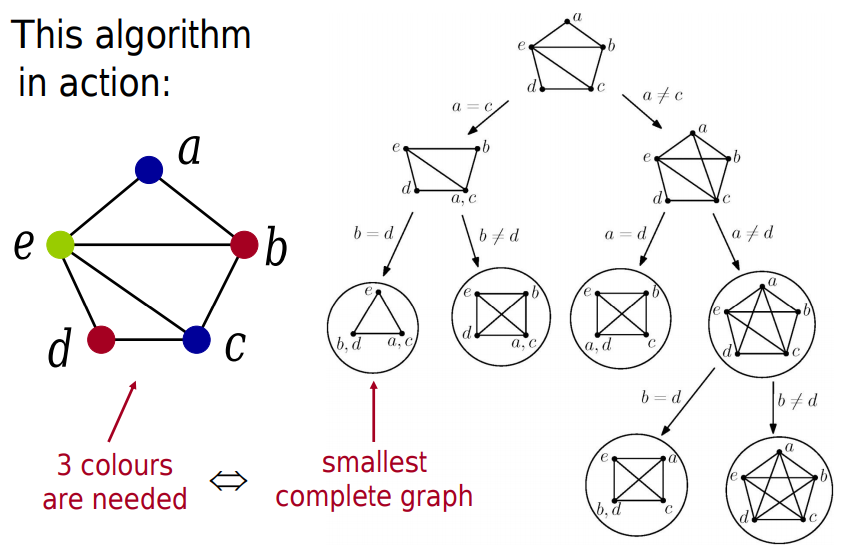
\includegraphics[scale=0.7]{inAction}
\end{center}
\begin{itemize}
\item However also this algorithm also has \textbf{exponential running time in the worst case}
\item This is called backtracking:
\begin{itemize}
\item try something (merge/add edge)
\item Then "undo" and try something else
\end{itemize}
\end{itemize}
\section{A different view of colouring}
If a graph can be coloured with \textbf{k colours}, then:
\begin{itemize}
\item each two vertices a and b with the same colour are not connected to each other, i.e.
\item The graph can be partitioned into k "colour classes" each having \textbf{no edges}
\end{itemize}
\begin{center}
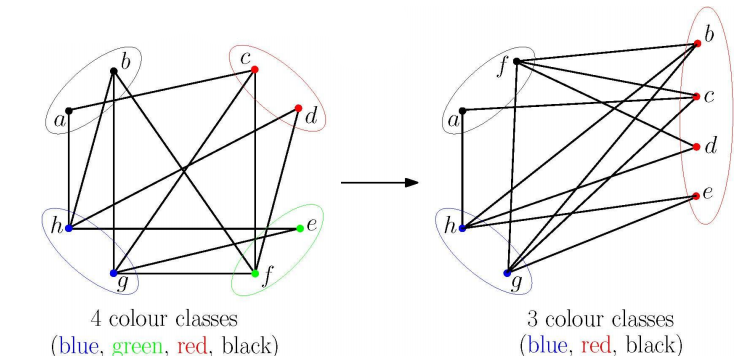
\includegraphics[scale=0.7]{classes}
\end{center}
Algorithmically, this formulation doesn't help much\\
\\
A graph is called k-partite, if it can be coloured with k different colours

\end{document}